We validate our approach of learning disentangle representations on several image datasets. The evaluation are mainly based on the quality of the samples from the model, the correlation analysis and classification accuracy on the learned representations. 

\subsection{Setup}
\paragraph{Data} We evaluate our methods on 3 image datasets: MNIST dataset~\footnote{http://yann.lecun.com/exdb/mnist/}, Face dataset~\footnote{http://www.multipie.org/} and Norb dataset~\footnote{http://www.cs.nyu.edu/~ylclab/data/norb-v1.0/}. MNIST contains 50,000 training and 10,000 testing samples from 10 different digit classes, and each image mainly contains two factors of variation: digit class and writing style. The face dataset contains the human face images from 68 persons with different lighting conditions and views, thus it provides 3 different factors. The norb dataset also contains 3 factors including category, rotation and brightness. 

\paragraph{Details} For each dataset, we convert the feature vector into normal distribution with mean zero and unit variance. We evaluate the performance on several models consists of different combinations of prior distribution and variational posterior distributions. The summary of the models are shown in Figure~\ref{table:model} The model A is the baseline from \cite{kingma2013auto}, Model B is trained with block diagonal posterior for variational distribution, and block diagonal prior with known block structure for prior distribution $p(\mathbf{z})$. The difference between Model B and C is that the Model C is trained with block diagonal covariance for variational distributions. Lastly, the Model D is the one trained with unknown block structure for covariance matrix. We evaluate and compare these models based on several criteria: a) 2-D cluster plot, this is the simplest way to see how each block structured. However, it only provides qualitative results and for larger dimensional latent representation, we have to do dimensionality reduction. b) we also evaluate the classification performance on the learned latent representations. i.e if the block captures the factor for digit class, we expect that we can have good classification performance by only looking at subset of hidden units which correspond to that particular factor. c) we also generate samples from the learned models, which will give us qualitative performance of our models. d) for learned hidden representations, we show the correlation matrix. In ideal case, this matrix should be in the form of block diagonal. In the following section, we provide empirical results for each dataset. 

\begin{table}
\centering
\begin{tabular}{|l|c|c|c|}
\hline
\backslashbox{Posterior}{Prior}  & N(0,1) & BLK & BLK(unknown) \\
\hline
 Diagonal& Model 1 & Model 2 & Model 4\\
 \hline
 BLK &  & Model 3& \\
% & all & all\\
\hline
\end{tabular}
\caption{The summary of the models used in this paper}
\label{table:model}
\end{table}


\subsection{MNIST datset}
\paragraph{Learn with 4 hidden units with 2 blocks}
For evaluation purpose, we assume the size of hidden units is $4$, and the input data has two factors. We define the covariance matrix for Model B and C as 4 by 4 matrix which includes two 2 by 2 submatrix in the diagonal. The same form applies to both prior and posterior variational distributions. Thus, for Model B and C, we know that the first two hidden units control the first factor and the remaining two hidden units control the second factor. However, for Model A, we don't know this beforehand, but we can still figure out the the subset of hidden units that correspond to first hidden factor and remaining sets control the second one, by doing greedy search (check all the combinations). Finally, for Model 4, we let the model to automatically discover the factors without defining the block structure. 

Figure[] shows the generated samples from four different models. The samples are generated by fixing one block while sampling another. We can see that...... By fixing one block, we actually select the mean sample from that distribution. Figure[] shows the clustering plots for each block. 
\textcolor{blue}{TODO: add generated samples,  plots. } 

\begin{figure}
\centering
	\begin{subfigure}[b]{1\textwidth}
    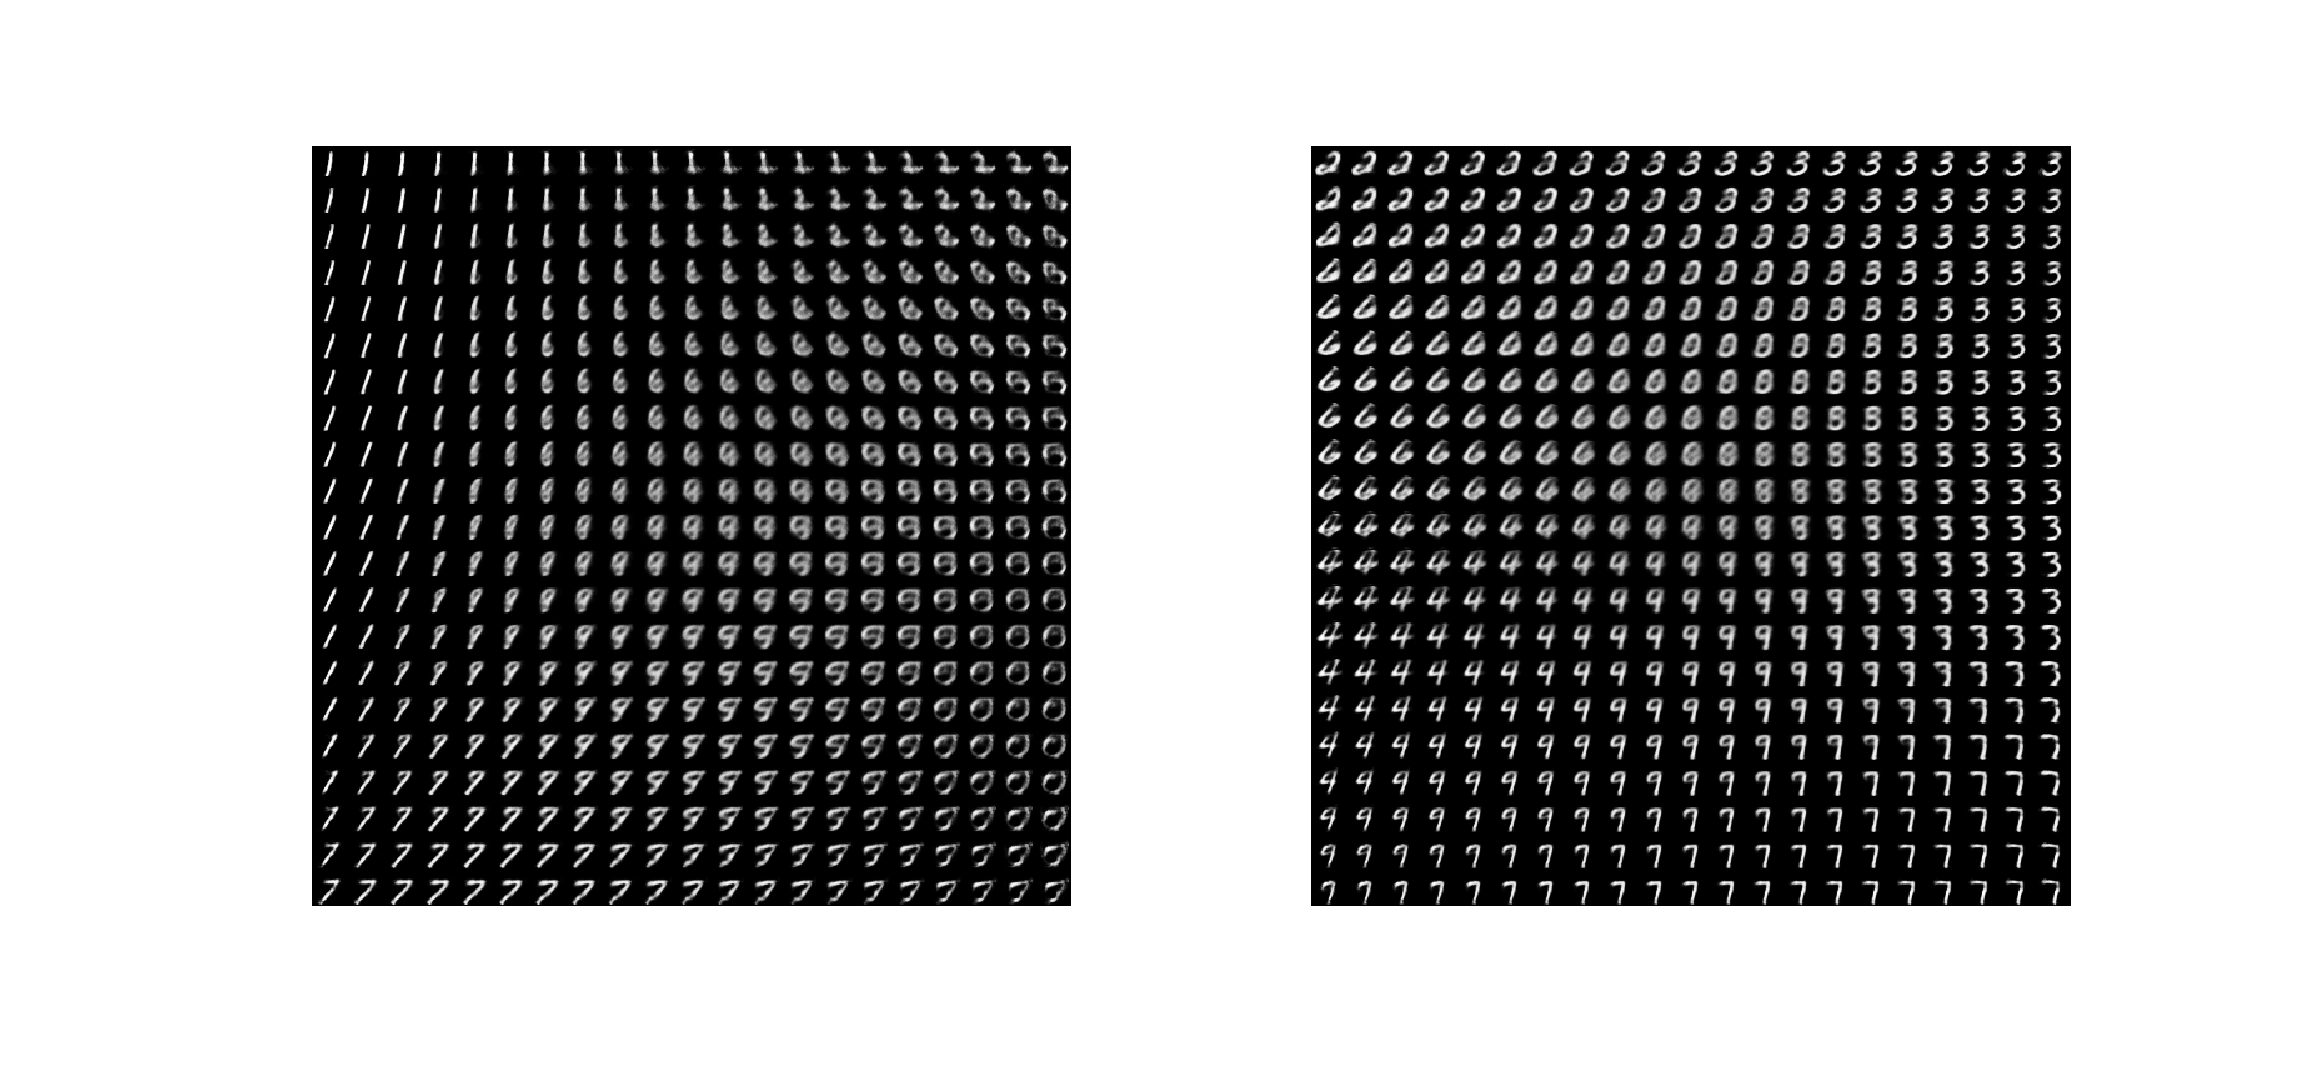
\includegraphics[width=\textwidth]{images/sampleNWdiag.eps}
    \caption{$p_{\theta}(\mathbf{z})$: block diagonal covariance with known structure $q_{\phi}(\mathbf{z}|\mathbf{x})$: diagonal variational posterior}
    \label{fig:us-air}
    \end{subfigure}
	~ %add desired spacing between images, e. g. ~, \quad, \qquad, \hfill etc.
          %(or a blank line to force the subfigure onto a new line)
    \begin{subfigure}[b]{1\textwidth}
    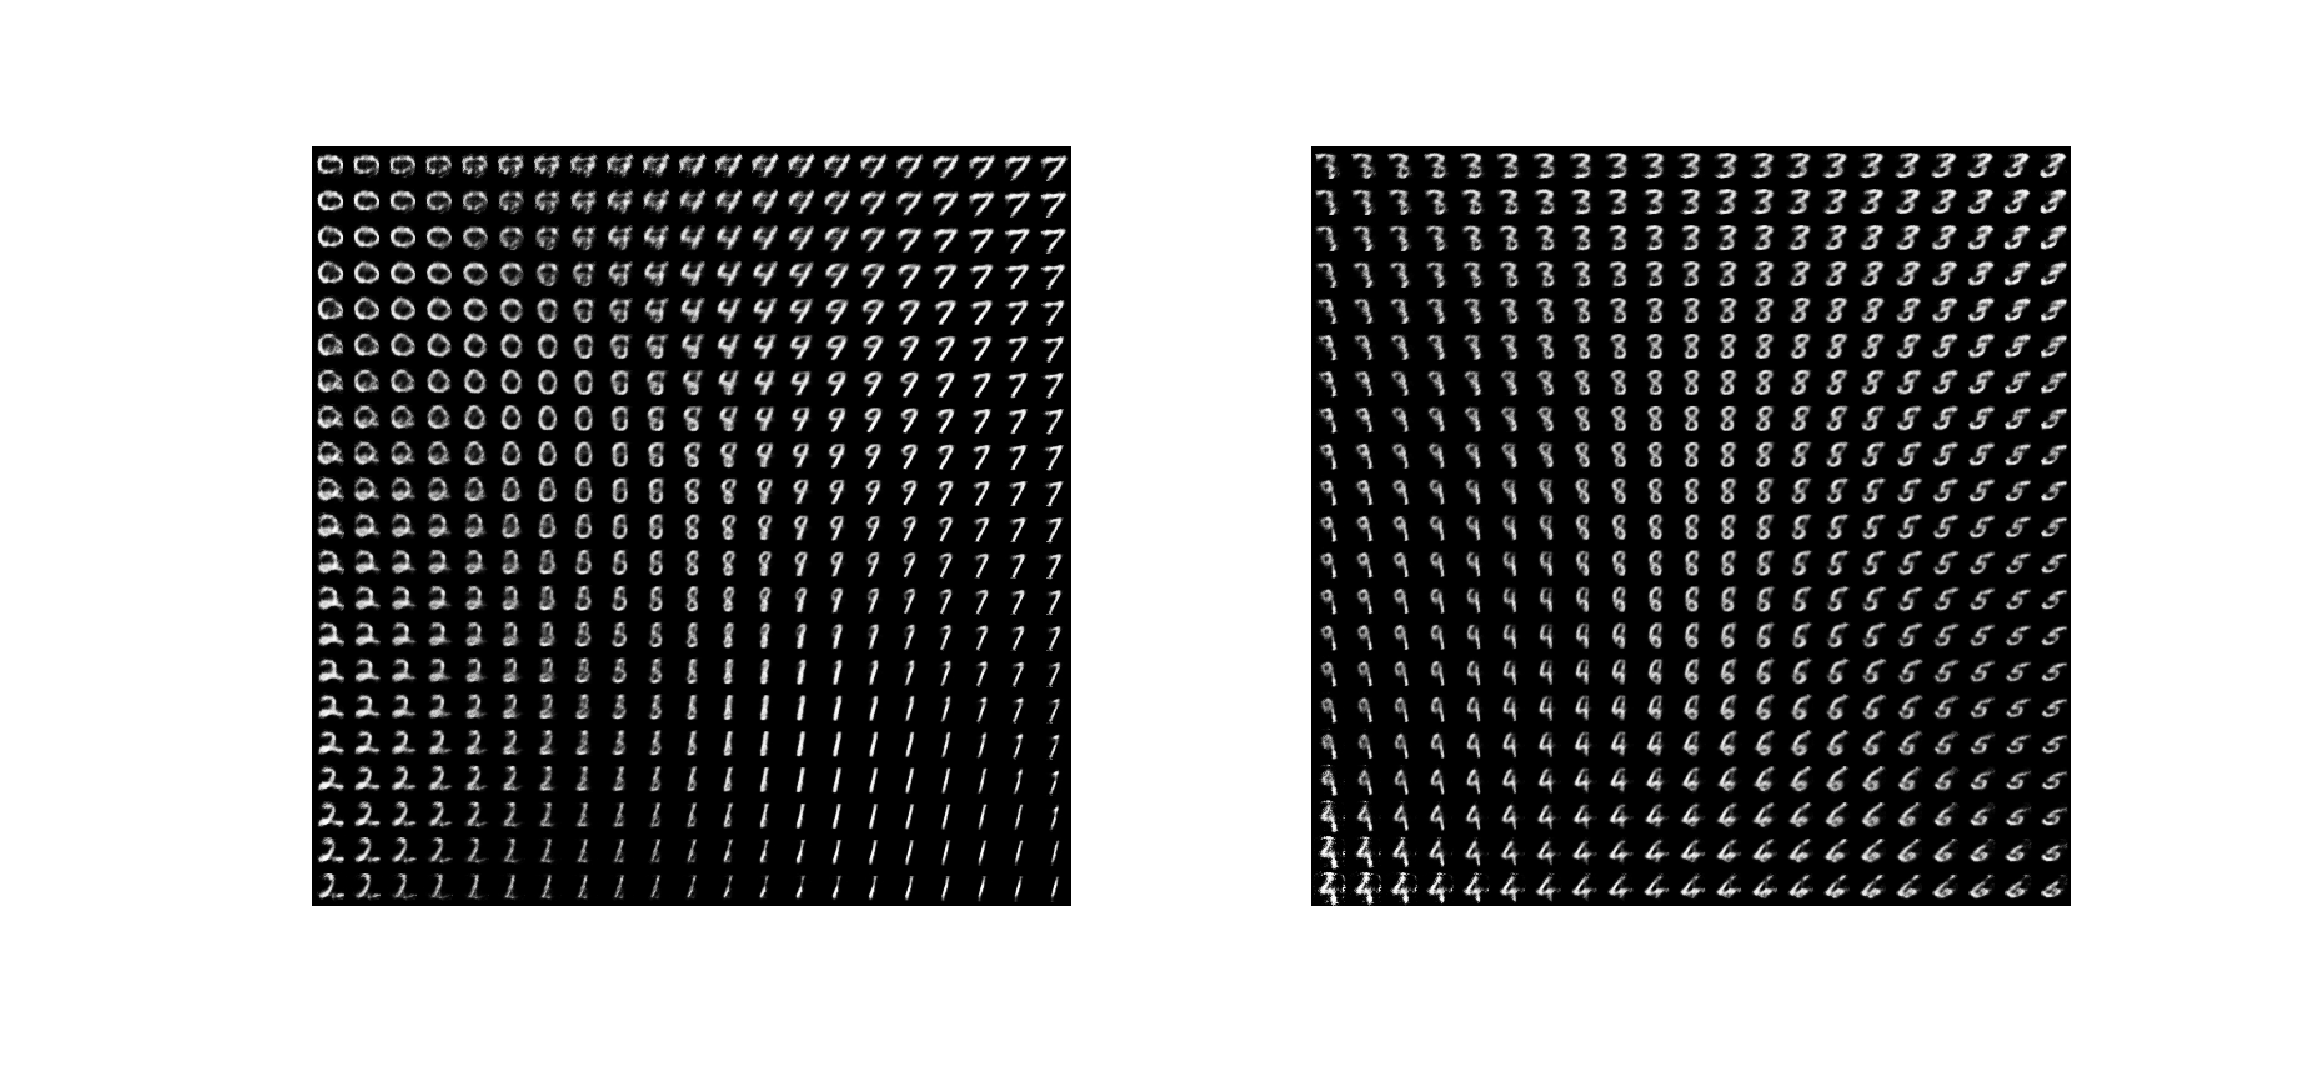
\includegraphics[width=\textwidth]{images/sampleNWblock.eps}
    \caption{$p_{\theta}(\mathbf{z})$: block diagonal covariance with known structure. $q_{\phi}(\mathbf{z}|\mathbf{x})$: block diagonal variational posterior}
    \label{fig:us-air}
    \end{subfigure}
    
    \begin{subfigure}[b]{1\textwidth}
    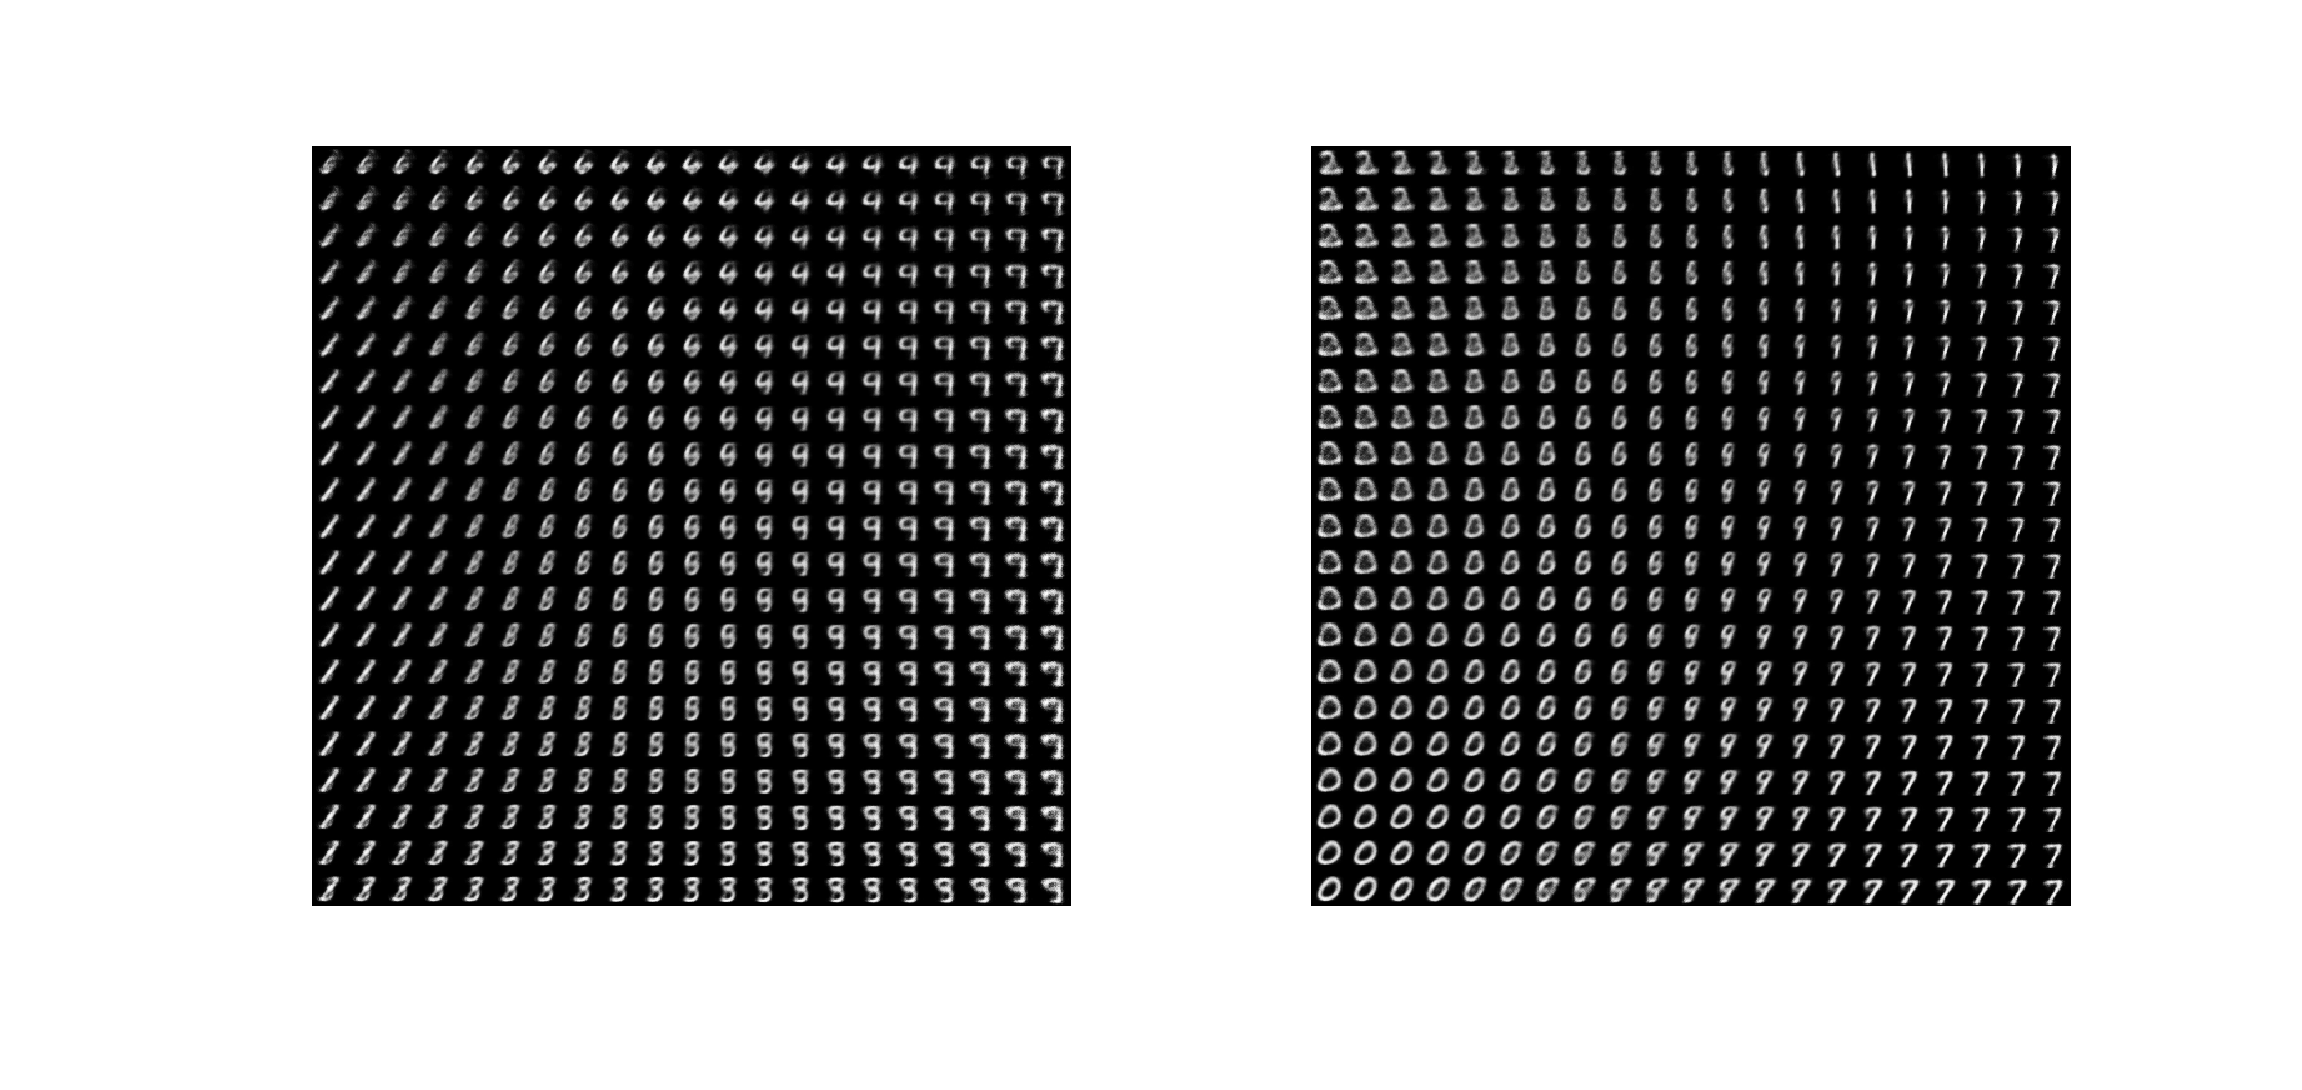
\includegraphics[width=\textwidth]{images/sampleAverage.eps}
    \caption{$p_{\theta}(\mathbf{z})$: block diagonal covariance with unknown structure. $q_{\phi}(\mathbf{z}|\mathbf{x})$: diagonal variational posterior}
    \label{fig:us-air}
    \end{subfigure}
    \caption{Generated samples from each block by fixing another, for three different models}\label{fig:animals}
\end{figure}


We also evaluate the predicative performance on the learned representation $\mathbf{z}$. For this purpose, we run the multinomial logistic regression on each block, and record the maximum accuracy between two (we expect that the factor encodes the digit class gives better prediction accuracy). Table[] shows the classification results on MNIST dataset by using learned latent representation as the input for the classifier. We can see that......
\textcolor{blue}{add classification table}

\begin{table*}[htb]
	\begin{center}
		\begin{small}
			\begin{sc}
				\begin{tabular}{lccc}
					\hline
					Data set & MNIST(2d)  & MNIST(10d) &   \\
					\hline
					Model 1& 53.9 & &\\
					Model 2 &44.4& &\\
					Model 3 & 56.7& &\\
					Model 4 & 48.2& &\\
					\hline
					% & all & all\\
				\end{tabular}
			\end{sc}
		\end{small}
        \vspace{0.2cm}
		\caption{Predictive performance on the 2D hidden representation which encodes the digit class factor}
\vspace{-0.5cm}		
\label{tab:regression}
	\end{center}
\end{table*}




\paragraph{Learn with 40 hidden units with 2 blocks}
For better understanding the correlation structure of learned representations, we plot the correlation matrix as in Figure[]. We can easily see that......  The prediction accuracy is also shown in Table[]. 
\textcolor{blue}{add correlation matrix plot}
\textcolor{blue}{add classification result table}


\subsection{Norb dataset}
In order to better understand the performance of our models. We also evaluate them on more complex datasets, which has three factors of variation. We use [] hidden units and we set the number of blocks to 3.  The Figure[] shows the generated samples from Model B,C,D. \textcolor{blue}{generated samples from Norb}. The correaltion matrix is also given in Figure[]. \textcolor{blue}{correlation matrix for Norb}  

\subsection{Face dataset}
We do the similar experiments as Norb dataset, with [] hidden units. Also, the face dataset contains three factors of variation. The Figure[] shows the generated samples from the learned models. \textcolor{blue}{generated samples from face dataset}, and Figure[] shows the correlation matrix. \textcolor{blue}{correlation matrix for face dataset}


